\chapter{Theoretical Foundations}\label{ch:theoretical-foundations}


\section{Sheet Metal}\label{sec:sheet-metal}
% Definition
Sheet metal is usually manufactured by flat rolling any type of metal and thus characterized by
its aspect ratio of surface area thinkess which is typically ranging from 0.4 mm to 6mm.
Above this range, its is considered to be a plate and below it is considered to be
foil~\cite[p. 405]{groover_fundamentalsmodernmanufacturing_2020}.
% Material
Low-carbon steel is the most commonly used type of sheet metal because it is low cost and has a good form ability as
well as its sufficient strength for most applications~\cite[p. 405]{groover_fundamentalsmodernmanufacturing_2020}.
% Commercial importance
Sheet metals play a vital role in many industries for example automotive and aerospace to reduce the weight of
products~\cite[pp. 1]{zheng_reviewformingtechniques_2018}.

\subsection{Sheet Metal Manufacturing}\label{subsec:sheet-metal-manufacturing}
% Manufacturing methods
Sheet metal working is primarily carried out using machine tools known as presses and the process
is referred to as sheet-metal press-working.
To carry out this processes stamping presses are used which are equipped with punch and die
tooling which is specifically designed for this purpose
\cite[p. 405]{groover_fundamentalsmodernmanufacturing_2020}.
The punch is a shaped tool that is usually mounted as upper part on the press ram and applies
pressure on the sheet metal to shape it.
The die is a stationary tool that is mounted in the press bed and provides a support surface for
the sheet metal and also defines the shape of the finished
product~\ref{sec:bending}~\cite[p. 412]{groover_fundamentalsmodernmanufacturing_2020}.
Figure~\ref{fig:bending-methods} shows the tooling setup together with a sheet metal being bend.

While the term `punch' is quite intuitive, the term ``die'' can cause confusion.
The term `die' is a typically term in metal working to refer to the lower or stationary part of a tooling setup.
It originated from old English word `dēag' which means a mold, shape, or form most likely refers to the fact that
the metal placed on the die is pressed or molded into a specific shape.

The sheet metal forming processes can be classified into three main categories: cutting, bending, and drawing.
The process of cutting is employed to divide large sheets of material into smaller pieces while bending and drawing
techniques are employed to shape sheet metal into the desired forms required for creating specific
parts~\cite[pp. 405]{groover_fundamentalsmodernmanufacturing_2020}.
Drawing involves stretching the metal to create a convex or concave shape, while bending involves strining the metal
to create a permanent bend.
The bending method used in this study (Air Bending) deploys a mixture of bending and drawing and will be
explained in more detail in the next section~\cite[pp. 416]{groover_fundamentalsmodernmanufacturing_2020}.


\section{Sheet Metal Bending}\label{sec:bending}
% Bending definition and description
Bending is a forming operation that is used to change the shape of a sheet metal by
apply a load to it.
It involves using force to shape the sheet mal in into a desired form~\cite[p. 1]{dib_singleensembleclassifiers_2020}.
The load is applied in way that exceeds the yield strength of the metal, but is below its
ultimate tensile strength, which allows the metal to bet permanently deformed into a
new shape~\cite[p. 1]{baig_machinelearningprediction_2021}.
A load below the yield strength will not deform the metal, while a load above the ultimate tensile strength will
cause the metal to break.
Sheet metal bending is usually used to produce large quantities of components at low cost in various
industries~\cite[p. 1]{dib_singleensembleclassifiers_2020}.

During the bending process, the metal sheet undergoes plastic deformation, where the outer fibers are stretches while
the inner fibers are compressed.
This results in a curvature of the sheet metal in the direction of the applied
load~\cite[p. 3]{baig_machinelearningprediction_2021}.
The bending process creates a neutral plane, which an imaginary surface within the metal sheet where there is
neither compression nor stretching.
It is also called neutral axis or neutral line~\cite[pp. 67]{gustafson1998analytical}.
Figure~\ref{fig:neutral-plane} shows the neutral plane after the bending operation, it is
visible, that it is closer to the inside of the bend than to the outside of the bend.
The arrows show where the metal was stretched and where it was compressed.

\begin{figure}[h]
    \begin{tcolorbox}[arc=0pt,boxrule=0.5pt, colback=white]
        \centering
        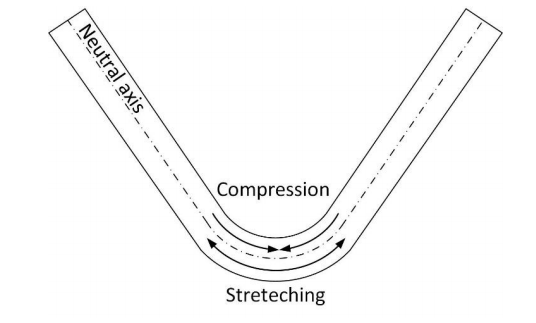
\includegraphics[width=0.6\textwidth]{chap2/images/neutral-plane}
    \end{tcolorbox}
    \caption{Bending plane, compression and stretching of sheet
    metal~\cite[p. 3]{baig_machinelearningprediction_2021}}
    \label{fig:neutral-plane}
\end{figure}

% How curvature is achieved 
The amount of curvature that is achieved in the bending process is determined by the
amount of load applied, the thickness and properties of the metal and the location and length of the neutral plane.
By controlling these factors, it is possible to achieve precise and consistent results in the bending of sheet metal.

\subsection{Air Bending}\label{subsec:air-bending}
Sheet metal bending is a fundamental process in the manufacturing industry, allowing for the creation of various
metal shapes and configurations.
V-bending and its variant, Air Bending, are common techniques that utilize punch-and-die
tooling~\cite[p. 416]{groover_fundamentalsmodernmanufacturing_2020}.

The V-bending process, as shown in Figure~\ref{fig:v-bending}, entails pressing the metal into the shape of the die
to form precise and complex bends.
The die can take various shapes, including U-shaped, Z-shaped, or any other shape required to achieve the desired bend.

In contrast, air bending, as depicted in Figure~\ref{fig:air-bending}, utilizes an open die that only supports the
metal on each side. This process permits a more extensive range of bend angles since the punch travel distance is not
restricted by the die. Air bending can also achieve a tighter bend radius compared to V-bending, but it may result in
a slightly rounded bend.

\begin{figure}[h]
    \begin{tcolorbox}[arc=0pt,boxrule=0.5pt, colback=white]
        \centering
        \begin{subfigure}{0.3\textwidth}
            \centering
            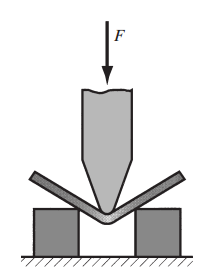
\includegraphics[width=\textwidth]{chap3/images/air-bending}
            \caption{Air bending}
            \label{fig:air-bending}
        \end{subfigure}
        \hfill
        \begin{subfigure}{0.3\textwidth}
            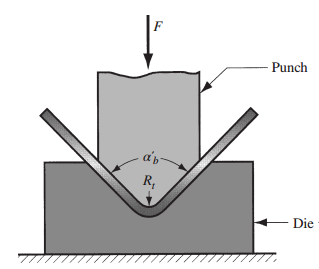
\includegraphics[width=\textwidth]{chap3/images/v-bending}
            \caption{V-Bending}
            \label{fig:v-bending}
        \end{subfigure}
        \hfill
    \end{tcolorbox}
    \caption{Differnt bending methods~\cite[pp. 416]{groover_fundamentalsmodernmanufacturing_2020}}
    \label{fig:bending-methods}
\end{figure}

% Usage of air bending
Air bending is commonly used in automotive industry to manufacture sheet metal
parts~\cite[p. 342]{kim_predictionbendallowance_2007}.
It is typically the preferred bending method because, its high flexibility because it
is possible to achieve different bending angles using the same punch-and-die
tooling~\cite[p. 3]{miranda_formingspringbackprediction_2018}\cite[p. 1]{cruz_applicationmachinelearning_2021}

% Pado: What’s a press brake bending machine?
Today press machines are usually equipped with ``copmputer numeral control (CNC) systems that can automatically
control the bending process and
produce the desired shape''~\cite[p. 3]{miranda_formingspringbackprediction_2018}
The process parameters and their are explained in the section~\ref{sec:process-parameters}.

\subsubsection{Spring Back}\label{sec:spring-back}
% How the spring back is created
After the deformation pressure from process described in section~\ref{subsec:air-bending} is released, there is still
some elastic energy remaining in the bent part.
As a result, the bent part will partially return to its original
shape, which is known as spring back~\cite[p. 413--414]{groover_fundamentalsmodernmanufacturing_2020}.

Figure~\ref{fig:spring-back} shows the spring back of a metal plate after the punch was removed.
The spring back is determined by the angle of the bent part after the bunch is removed compared to the angle when
the punch was still applied.
The solid line shows the metal plate in its original form when the punch was still
applied. The dashed line shows the metal plate after the punch was removed.

\begin{figure}[ht]
    \centering
    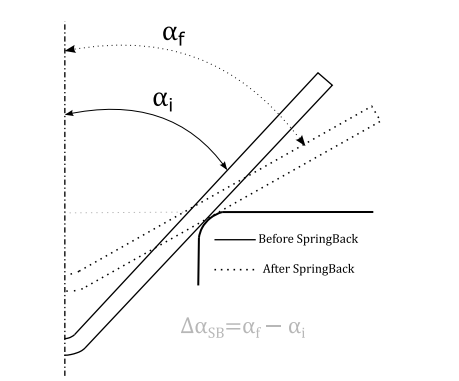
\includegraphics[width=0.5\textwidth]{chap3/images/spring-back}
    \caption{Spring back~\cite[p. 5]{cruz_applicationmachinelearning_2021}}
    \label{fig:spring-back}
\end{figure}

The angle before the spring back is usually denoted as $\alpha_f$ and the angle after spring back as $\alpha_i$.
% Introduce of formula
The spring back ($\Delta \alpha_{SB}$) is therefore the difference between $\alpha_f$ and
$\alpha_i$ as show in equation~\ref*{eq:calculation_springback}~\cite[p. 6]{cruz_applicationmachinelearning_2021}.

\begin{equation}
    \delta \alpha_{SB} = \alpha_i - \alpha_f
    \label{eq:calculation_springback}
\end{equation}

To tackle this problem, there are various techniques to compensate for spring back.
One commonly used approach is over bending, wherein the punch angle and radius are fabricated smaller than the
specified angle.
Prerequisite for all compensation methods is that the spring back is known therefore
the accurate prediction of the spring back play an important role in the manufacturing
process ~\cite[p. 114]{groover_fundamentalsmodernmanufacturing_2020}.


\section{Machine Learning}\label{sec:machine-learning}
The concept of machine learning involves deriving insights and information from data.
It is a scientific discipline that sits at the crossroads of computer science, artificial intelligence, and statistics,
and is sometimes referred to as predictive analytics or statistical
learning~\cite[p. 1]{muller_introductionmachinelearning_2016}.

Machine learning algorithms create a model by analyzing a sample dataset, commonly known as training data. The
purpose of the model is to make predictions or decisions without requiring explicit programming to perform the task.
These algorithms rather than being `hard coded' they are `soft coded' meaning that they adapt their structure
automatically though repetition to improve their performance in achieving the desired task~\cite[pp. 4]{el2015machine
}~\cite[pp. 151--170]{koza1996automated}.
This adaptive process is called training, in wich input data samples are provided along with desired outcomes,
allowing the algorithm to optimize itself to produce the desired result not only with the training inputs but also with
new, previously unseen data~\cite[pp. 4]{el2015machine}.
The process producing reulsts on unseen data is also called generalization~\cite[p. 4]{zhou_machinelearning_2021}.
The training is the fundamental aspect of \ac{ML} and it can be continuous allowing the algorithm to
learn from new data and its mistakes~\cite[pp. 4]{el2015machine}.

Machine learning algorithms have numerous applications in fields just as example agriculture (\cite{
    yoosefzadeh2021application}), computer vision (\cite{hu2020voronoi}) or metal working
(see section~\ref{sec:state-of-research}).

\subsection{Terminology}\label{subsec:terminology}
To carry out machine learning, a \textit{dataset} is required as the initial foundation.
A dataset is composed of \textit{samples}, with each sample being a single row or observation.
For example, if a dataset contains information about metal sheet bending, each row would represent a single bend.

A \textit{feature} is an individual measurable property or characteristic of the data, and the associated value is
called
an \textit{attribute}.
A feature could be, for example, the thickness of a sheet metal component, and the attribute could be 3mm.
Features used to predict the outcome of a sample are called \textit{independent features}, while the outcome feature is
referred to as the \textit{dependent feature} or \textit{target}. In this study, the springback is the dependent
feature.
The dataset of this study will be explained in section~\ref{subsec:dataset-exploration}.

The process of using machine learning algorithms to create a model is called \textit{training}, and the data used for
that process is referred to as \textit{training data} or \textit{fitting}.
Usually, the training data is a subset of the whole dataset.
The process of using the model to make predictions on new, unseen data is called
\textit{generalization}~\cite[p. 35]{muller_introductionmachinelearning_2016}.
The test-train split is described in more detail in section~\ref{subsec:test-train-split}.

The outcome of the learning process is referred to as a \textit{model} that can be used to make predictions on new,
unseen data.
\ac{ML} algorithms are also often reffered as \textit{learners}.

\subsection{Supervised Learning and Unsupervised Learning}\label{subsec:supervised-learning}
Learning tasks can be categorized in two groups, based on whether the training data already contains the outcome or not.
These groups are supervised learning and unsupervised learning~\cite[p. 4]{zhou_machinelearning_2021}.

Supervised learning is employed when not only the independend features but also the dependent feature is known.
Since this is the case in the dataset used in this study, supervised learning is the preferred
method~\cite[p. 25]{muller_introductionmachinelearning_2016}.
To achieve this supervised \ac{ML} algorithms are trained with parts of the dataset, the training data.
Building the trainin set usually requires human effore but once it is built supervised learning automates the task
and makes it more efficient. The two main types of supervised learning are classification and
regression~\cite[p. 25]{muller_introductionmachinelearning_2016}, which will be explained in the following section.

\subsection{Classification and Regression}\label{subsec:regression}
There are two main types of supervised machine learning problems: classification and
regression.
For regression tasks it is the goal to predict a continuous numerical value.
This can be a real number in mathematical terms or a floating-point number in programming
terms~\cite[p. 226]{muller_introductionmachinelearning_2016}
Classification problems involve predicting a class label, which is a choice from a
predefined list of possible options~\cite[p. 25]{muller_introductionmachinelearning_2016}.

% Examples
An example for a classification problem could be the prediction of the type of a flower based on its features such as
petal length and width. The possible outcomes are the different types of flowers, which are the class labels.
The class labels are discrete values, which means that they are not continuous.
An example for a regression problem could be the prediction of the price of a house based on its features such as
number of rooms and square footage. The possible outcomes are the different prices of houses, which are the
continuous values.

Since spring back is a continues values usually expressed in millimeters or degrees, this study focuses on
regression problems.

\subsection{Empirical Error and Overfitting}\label{subsec:overfitting-and-underfitting}
The discrepancy between the output predicted by the learning algorithm and the actual output is referred to as the
error.
The error computed on the training set is known as training error or empirical error, while the error determined on new
samples is called generalization error~\cite[p. 26]{zhou_machinelearning_2021}.
The goal of machine learning is to minimize the generalization error.
The difficulty is, that the details of new samples are unknown while training the learning algorithm, that means that
only the empirical error can be minimized.
This bears the risk of creating models that perform well on the training data but
generalize poorly on new, unseen data.
A usual reason is that the algorithm learns details of the training samples as general properties of the data
which are not true for new samples.
This phenomenon is called overfitting and is the main reason why the generalization error is usually higher than the
empirical error.
The opposite phenomenon is called underfitting and happens when the algorithm fails to learn geneal properties of
the training samples~\cite[p. 26]{zhou_machinelearning_2021}.

An overfitting model is too complex for the amount of information available and therefore does not generalize well,
while an underfitting model is too simple an does not perform well on the training set.
Complex in this context means, that the model has a high number of parameters, which get adjusted in a way while
training the model that it fits the training data too well.

As an example for overfitting, consider a model that tries to predict the price of a house based on its square footage.
The model could learn that the price of a house is proportional to its square footage, but it could also learn that the
price of a house is proportional to its square footage plus the number of rooms.
The latter model would overfit the training data, because it would not generalize well to new samples.

\textit{Or should I use a picture as example of overfitting?}

The goal is to find the simplest model that captures the variability in the
data~\cite[p. 35]{muller_introductionmachinelearning_2016}.

\subsection{Bias-Variance Tradeoff}\label{subsec:bias-variance-tradeoff}
Aside from determining the generalization ability of learning algorithms, it is also usefull to comprehend the
reasons behind the performance.
A crucial mechanism for comprehending the generalization performance of algorithms is the bias-variance
decomposition~\cite[pp. 49]{zhou_machinelearning_2021}.

Bias measures the difference between models predictions and the actual
(ground-truth) values~\cite[p. 51]{zhou_machinelearning_2021}.
It measures how well the model can capture the underlying
relationships~\cite[p. 7--8]{neal_biasvariancetradeofftextbooks_2019}.
A model with high bias is typically too simple and therefore unable to capture the complexity of the data, resulting
in underfitting.
On the other hand, a model with low bias is typically too complex and therefore can capture better the underlying
patterns in the data. But if the model gets too complex it will result in
overfitting~\cite[p. 20]{neal_biasvariancetradeofftextbooks_2019}.

The term `variance' refers to the variability in the learning performance cause by changes in the training
set~\cite[p. 51]{zhou_machinelearning_2021}.
A model with low variances typically generalizes well on new data while high variance indicates that the model
overfits the training data and therefore does not generalize well on new
data~\cite[p. 7--8]{neal_biasvariancetradeofftextbooks_2019}.

Variance and bias are conflicting because the represent two different sources of error.
Error from bias is due to the model being too simple, while error from variance is due to the model being too
complex.
Therefore, as the model becomes more complex, the bias decreases and the variance increases, and vice versa.
This is known as the bias-variance tradeoff and the coal is valled to find a model that strikes the balance between
bias and minimizes the overall error of the model on new unseen
data~\cite[p. 9]{neal_biasvariancetradeofftextbooks_2019}.


% Regularization
%\subsubsection*{Regularization}
%Regularization refers to a group of techniques that force a model to be simpler.
%this usually results in a slight increase in bias but a substantial decrease in
%variance~\cite[p. 12]{burkov2019hundred}.
%
%The regularization method used in this thesis and in general the most popular are L1
%and L2 regularization.
%In order to construct a regularized model, the objective function is altered by
%including a penalizing term that increases the value as the model becomes more complex~\cite[p. 12]{burkov2019hundred}

%\subsection{Ensemble Learning}\label{subsec:ensemble-learning}
%Ensemble techniques in machine learning to involve the construction of multiple models
%, called
%"learners," for a given task. The primary goal of these methods is to improve the
%accuracy and
%performance of the model by combining the predictions of multiple learners. Ensemble
%techniques
%differ from single classifier methods by constructing multiple models and combining
%them using a
%voting strategy in order to highlight different aspects of the data. This can
%potentially lead to
%improved overall performance. \cite[p. 253]{shaik_briefsurveyrandom_2019}

\subsection{Evaluation and Improvements of Models}\label{subsec:evaluations-and-improvements-of-models}

\subsubsection{Cross Validation}\label{subsubsec:cross-validation}
Cross-validation is a method of evaluating the performance of a model by training
multiple models on different subsets of the data and evaluating their performance.
The most common version of cross-validation is k-fold cross-validation, in which the data is divided into k folds,
and k models are trained, each using a different fold as the test set and the remaining folds as the training set.
The accuracy of each model is then evaluated, and the average accuracy across all k
models is used as an estimate of the generalization performance of the model.
This process helps to reduce the variability in model performance due to the specific choice of training and test
sets, and is therefore considered to be a more stable and reliable way to evaluate the performance of a
model~\cite[p. 252--260]{muller_introductionmachinelearning_2016}.

Figure~\ref{fig:cross-validation} shows how the cross-validation process and how the variance
is calculated.
It can be seen that the training data set was divided into multiple folds.
The number of folds is denoted as $k$.
One fold is used as test set (grey) while the remaining folds are used as training set (white).
A model is trained on each iteration and the performance is evaluated with a metric denoted as $E$.
Common metrics that can be used for evaluation are $R^2$, $MSE$, $MAE$ and $RMSE$ which are explained in section
\ref{sec:dp1:-correctness} where they are used.

\begin{figure}[h]
    \begin{tcolorbox}[arc=0pt,boxrule=0.5pt]
        \centering
        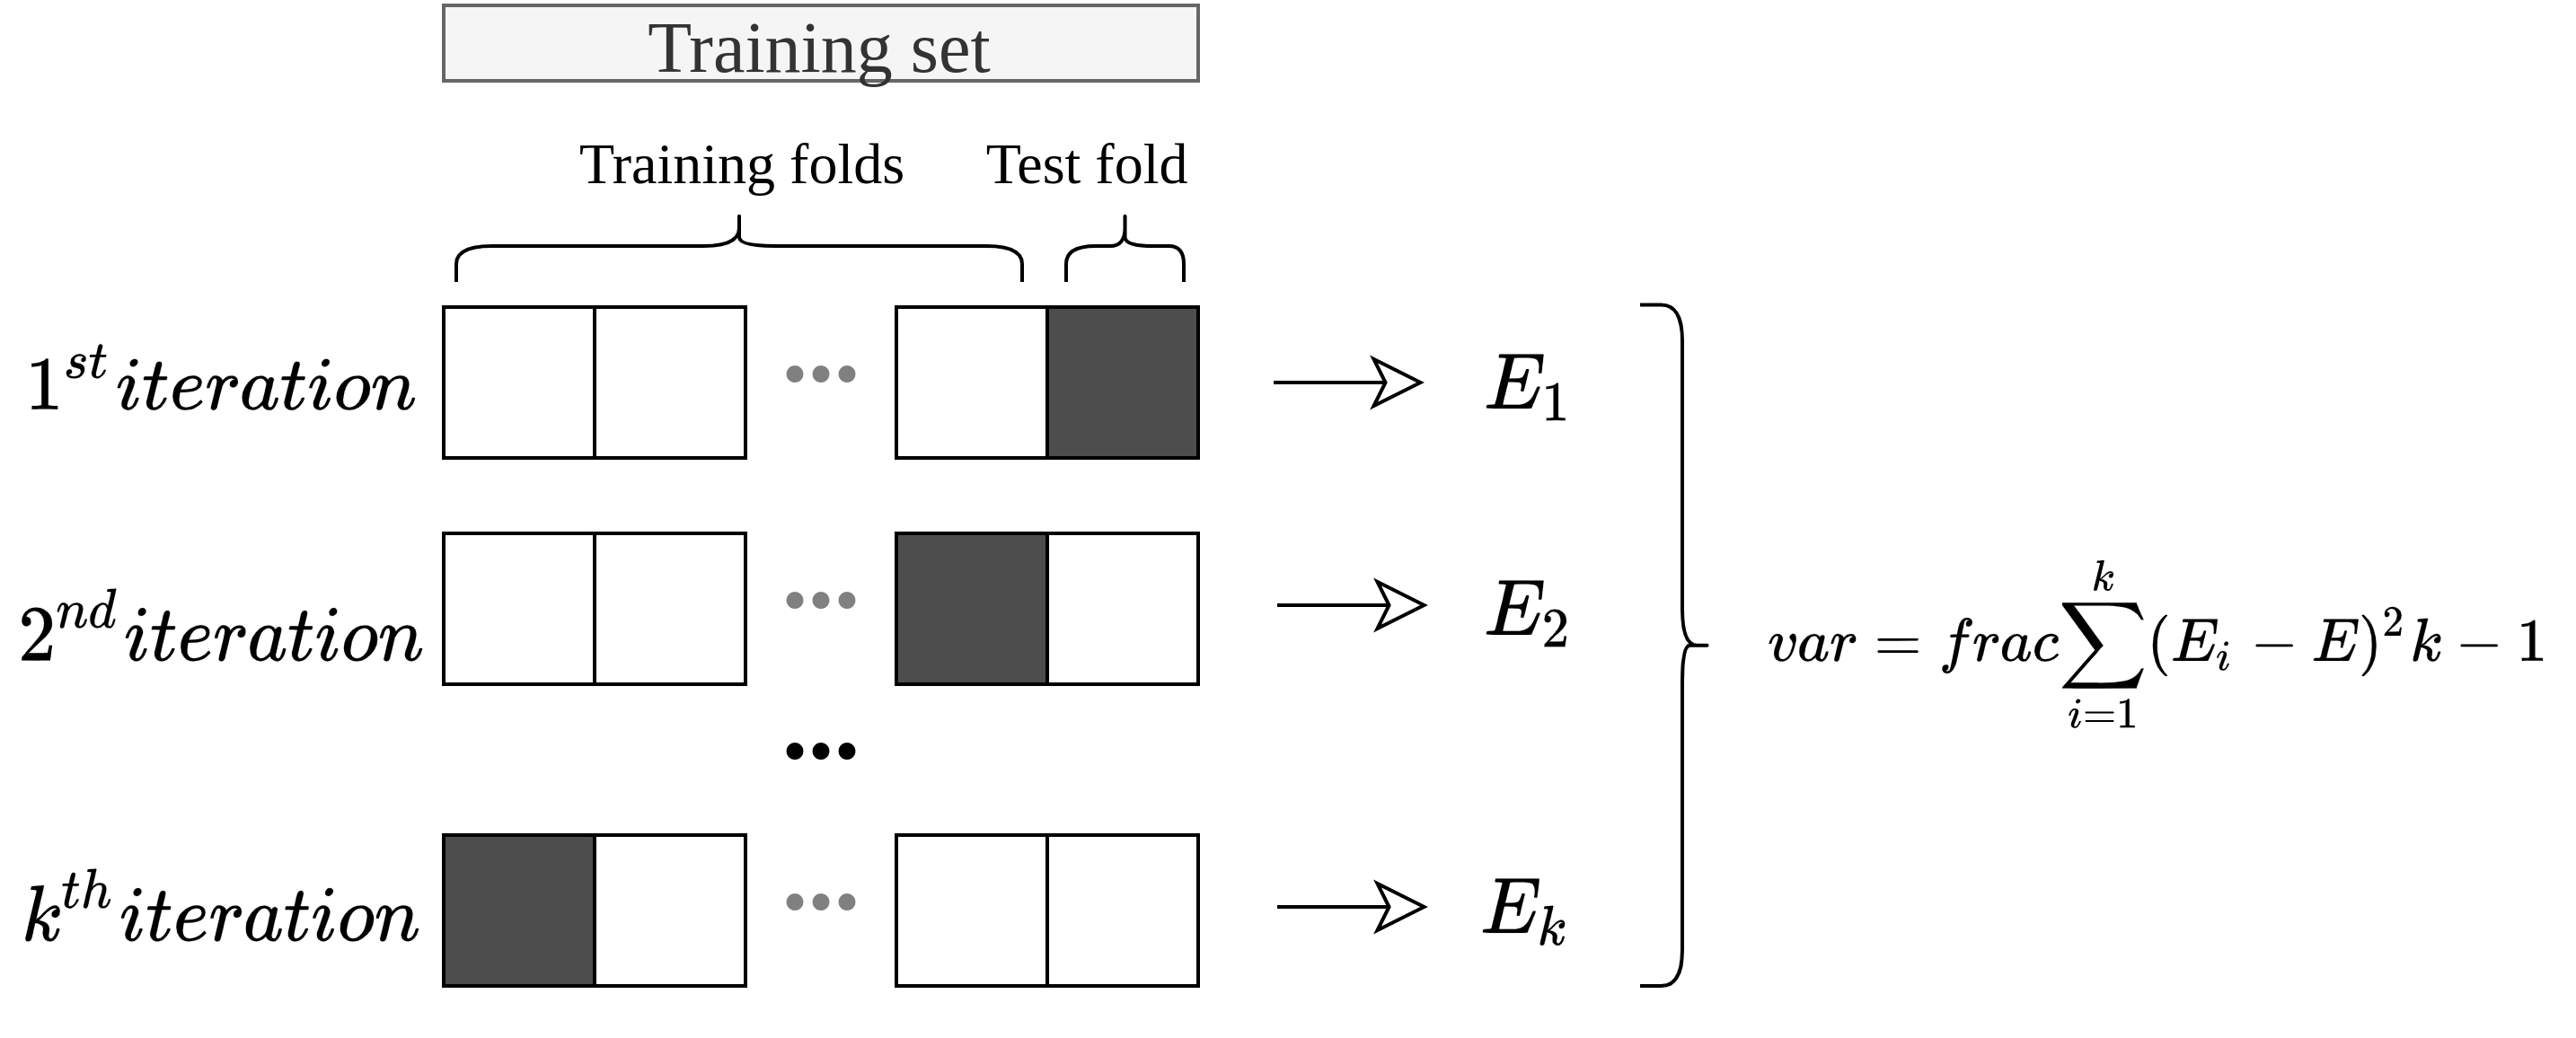
\includegraphics[trim=left botm right top, width=0.9\textwidth]
        {chap2/images/cross_validation}
        \caption{Variance of cross-validation}
        \label{fig:cross-validation}
    \end{tcolorbox}
\end{figure}

\subsubsection{Grid Search}\label{subsubsec:grid-search}
Each machine learning method has a number of parameters that can be tuned to improve the
performance of the model.
Parameters are often not known in advance and must be tuned to the data.
This is a common task in machine learning and therefore there are standard methods like
grid search to find the best parameters.
Grid search is a method of systematically working through multiple combinations of
parameters (called grid), cross-validating as it goes to determine which tune gives the best
performance~\cite[p. 260--275]{muller_introductionmachinelearning_2016}.


\section{State of research}\label{sec:state-of-research}
Sheet metals exhibit a high ratio of yield strength to elastic modulus, which leads to significant springback,
potentially compromising the accuracy of the final product. Consequently, extensive research has been conducted to
estimate spring back behavior in sheet metal forming processes~\cite[p. 565]{liu2021deep}.
In recent years, there has been a surge in the adoption of \ac{ML} for various applications related to sheet metal
forming, aiming to achieve optimal manufacturing quality. Both supervised and unsupervised \ac{ML} methods have been
employed in these applications~\cite[p. 2]{cruz_applicationmachinelearning_2021}.

Current research on mitigating spring back in sheet metal forming primarily focuses on compensation methods through
numerical simulations, most notably finite element analysis (FEA)\cite[p. 565]{liu2021deep}.
That means that the data used for training the model is generated by a simulation.

Lingbeek et al.\cite{lingbeek2005development} present two methods for compensating sprin gback in the deep
drawing process, but conclude that more reliable simulations are needed for industrial applications.
Liu et al. utilized an Support Vector Machine to predict spring back in a micro W-bending process, demonstrating high
prediction accuracy and generalization performance compared to experimental
results~\cite[p. 1]{liu_springbackpredictionforming_2019}.
Dib et al. evaluated several \ac{ML} algorithms for predicting spring back and maximum thinning in U-channel and square
cup forming processes, with the a Multilayer Perceptron emerging as the best
model~\cite{dib_singleensembleclassifiers_2020}.
Likewise, Abdessalem et al. compared the performance of a quadratic response surface method (RSM) and two \ac{SVM}
models for determining the best surrogate model for probabilistic structure optimization of sheet metals.
Both \ac{SVM} models outperformed the RSM model~\cite[]{abdessalem2015probabilistic}.

It has to be noted that most of the research including \ac{ML} relies on FEA to generate the data for training and
testing the models.
This is due to the fact that it is time consuming to obtain enough experimental data for
sheet metal forming processes.
Dib et al. note that the implementations of virtual tryout still heavily relies on human expertise to make critical
decisions.
Also the use of FEM does not necessarily eliminates unexpected defects due to variations
in material properties, tool geometry and process parameters~\cite[p. 2]{dib_singleensembleclassifiers_2020}.

\subsection*{Spring Back Prediction Using Unsupervised Learning}
\labelsub{subsec:spring-back-prediction-using-unsupervised-learning}
Artificial Neural Networks \ac{ANN}s are widely used in sheet metal forming because of
their high accuracy and generalization performance~\cite[p. 2]{cruz_applicationmachinelearning_2021}.
\cite[]{narayanasamy_comparisonregressionartificial_2012a} which compared regression
and neural network modeling for predicting spring back of steel sheet metal during the air bending process.
They observed that ANN was able to predict the spring back with higher accuracy. But
they had a sample size of 25 and suggested further research.
\cite[]{inamdar_developmentartificialneural_2000} developed an ANN for the air bending
process to predict spring back as well as the punch travel to achieve the desired angle in a single stroke.
\cite[]{kazan_predictionspringbackwipebending_2009} developed an ANN trained with FEM
simulation data to predict the spring back for the wipe-bending process.

Because \ac{ANN}s need a large amount of data to train the model generating the data
with real
machines is a time-consuming process.
Therefore, it is common to use \ac{ANN}s trained with Finite Element Method \ac{FEM}simulation data.

\textit{Was sind die Nachteile von FEM? Warum nutze eich "echte" Experimente?}
\subsubsection*{Spring Back Prediction Using Supervised Learning}
Liu et al. (2019) used a Support Vector Machine \ac{SVM} to predict the spring back of
micro
W-Bending operations~\cite{liu_springbackpredictionforming_2019}.
Dib et al. (2019) compared different \ac{ML} techniques (logistic regression, SVM, KNN
, ANN,random forest, decision tree, naive Bayes, MSP) to predict the spring back and the occurrence of
defects in sheet metal~\cite[p. 1]{dib_singleensembleclassifiers_2020}.
The authors conclude that the MLP and the SVM are the best performing algorithms and
suggest further studies of ML regressions models and kriging regression
models~\cite[p. 13]{dib_singleensembleclassifiers_2020}.

% Artificial neural networks, among the various types of learning algorithms, are widely
% used in sheet metal forming processes due to their ability to overcome the limitations
% imposed by nonlinearities and the multiple parameters involved in forming problems.
% Several articles on air bending have been published, following the use of artificial
% neural
% networks [23–27]. The authors of [28] studied the use of ANN on modeling the air V-
% bending processes using both an analytical and experimental data set and demonstrated
% the capability of ANN to model the springback problem. The authors of [29] implemented
% a neural network in order to predict the stepped binder force trajectory for
% different punch
% displacements, in a plane strain channel forming process. The authors of [30] evaluated
% the applicability of ANN to the problem of choosing a tool geometry to bend a component
% with a defined shape. A finite element model created to simulate the bending process
% and a genetic algorithm (GA) were used to optimize the weights of an artificial neural
% network, thus reducing the deviation between the predicted tool and the experimental
% solution. The authors of [31] analyzed the performance of a multilinear regression model
% and an ANN in predicting the springback angle in air bending processes. The results
% show ANN outperforming the regression models approach for the evaluated cases. The
% authors of [32] also investigated the effect of bending and springback angles in bending
% processes. In this case, experimental data obtained from FEA models was used to design
% and train the developed ANN models. The results confirm the validity of the FEA analysis
% and consequently their capability to provide data for developing ANN. The authors
% of [33] developed a combination of error backpropagation neural network and spline
% function (BPNN-Spline) in order to estimate the springback angle in a V-die bending
% process. The results showed that the proposed BPNN-Spline model outperforms the
% traditional ANN in predicting the bending angles for different punch displacements. The
% authors of [3] developed a methodology based on ANN and FEA, capable of establishing
% the specific punch displacement for bending a sheet metal material according to the
% desired forming angle in press brake bending. The results showed that the developed
% methodology can successfully predict the required punch penetration to achieve a given
% bending angle by considering results both for geometry after springback and also
% geometry
% before springback.


% To the best of the authors’
% knowledge, there are currently no studies available in the
% literature regarding ML classification focused on defect
% prediction in sheet metal forming processes under vari-
% ability, which is the main subject of the current work.
% \cite[]{dib_singleensembleclassifiers_2020}


% Baig
% \section{Bending allowance and k-factor}
% "As always, real-world materials do not behave as simply as our models. After the
% material has
% taken on its new shape in between the hardened steel tools of the press, this central
% neutral
% line will be pretty messed up by the interaction. We can’t really know the course of the
% neutral line after the bend without a detailed and rather complex model of the material
% characteristics. To make things easy, an imaginary neutral line based on a simplified
% approximation can be used to predict the length of the flat pattern:"
% "To do this, a correction factor, k, is introduced. The factor offsets the neutral
% line piece
% in the bend region from its center path until it has the length of the corresponding
% region of
% the flat pattern. The k-factor is empirically determined for a given material, material
% thickness, bend radius, and bending method. It reflects all real but unknown
% distortions in the
% bend region."

% "Since the k-factor depends on several factors, tables of empirically determined
% k-factors for
% given setups are used. Using the k-factor, we can now calculate the bend allowance
% "BA", which
% is the length of flat material that goes into the bend region. It’s simply the arc
% length of
% the "imaginary" neutral line piece, that has been offset by the k-factor:"
% "Of course, the approximation is only as realistic as the k-factor used, and it makes
% sense to
% keep your own table with k-values for the materials you intend to work with. However,
% the
% following values are a good starting point:"


% \section{Bend deduction}
% "In practice, the flat pattern length is always shorter than the sum of A and B, so
% everything
% above can be condensed in the difference between A + B and L, which is called the bend
% deduction "BD"."
% \cite{by_artsciencebending_2016a}

% “Die beim Biegevorgang stattfindende plastische Formänderung beschränkt sich dabei
% nicht nur
% auf eine reine Richtungsänderung, sondern es tritt gleichfalls eine plastische
% Änderung der
% Länge auf. So wird die dem Werkzeug zugewandte Seite des Biegeteils gestaucht,
% während die
% gegenüberliegende Seite eine Verlängerung infolge Dehnung erfährt. Dieses Verhalten
% während des
% Umformprozesses wird als Biegeverkürzung oder auch als Biegezugabe bezeichnet, je
% nachdem,
% welche Seite des Biegeteils man betrachtet.”
% \cite{rockhausen_integrationsolidworksprozesskette_2010} 

% “Dabei ist diese plastische Verformung keineswegs linear und ihre Berechnung nicht
% trivial. Die
% Biegezugabe stellt einen Zahlenwert dar, der von mehreren Faktoren abhängig ist, so zum
% Beispiel vom Material, von der Blechdicke und den verwendeten Werkzeugen. Zwar gibt
% es hierfür
% Formeln zu ihrer Berechnung, so zum Beispiel nach DIN 6935, doch auch diese
% approximieren nur
% die in der Fertigung tatsächlich auftretenden Biegezugaben. Daher werden oft
% Erfahrungswerte
% zugrunde gelegt, die oftmals die zuverlässigere Annäherung darstellen.”
% \cite{rockhausen_integrationsolidworksprozesskette_2010} 

% springback is entirely intercorrelated with the stress distribution on sheet metal as
% residual
% stresses [42]. Its behavior is also affected by material properties such as strain
% hardening,
% elastic property evolution, the presence of Bauschinger effects, elastic and plastic
% anisotropy, and tribology between contacting surfaces [43]. Although there are
% mathematical
% models for predicting springback in bending situations, most of them are simplistic
% and do not
% take into account all influential factors.” (Cruz et al., 2021, p. 4)

% \section{}{Machine Learning}
% "Machine learning is a branch of Artificial intelligence in which, given input data
% points and
% output value, a computer algorithm learns rules by Analyzing the data. In other
% words, it gives
% systems the ability to learn and improve themselves without explicitly being
% programmed. The
% recent advancement in technology and the development of manufacturing 4.0 also
% triggered the
% need for machine learning. It means that the machines are producing data at an
% unprecedented
% scale, so now it is needed to have fast learning algorithms that can give accurate
% results in a
% short amount of time. This need triggered engineers worldwide to build new sets of
% algorithms
% that are fast at learning and can also give reliable answers. One such group of
% algorithms
% already exist which are known as tree-based learning algorithms. A tree-based learning
% algorithm is a group of machine learning algorithms that are used for supervised
% learning."
% \cite{baig_machinelearningprediction_2021}

